%% PNAStwoS.tex
%% Sample file to use for PNAS articles prepared in LaTeX
%% For two column PNAS articles
%% Version: Apr 15, 2008 
 

%% BASIC CLASS FILE
\documentclass{pnastwo}

%% ADDITIONAL OPTIONAL STYLE FILES
\usepackage[dvips]{graphicx}
%\usepackage{pnastwoF}
\usepackage{amssymb,amsfonts,amsmath}


%% OPTIONAL MACRO DEFINITIONS
\def\s{\sigma}


%%%%%%%%%%%%
%% For PNAS Only:
\url{www.pnas.org/cgi/doi/10.1073/pnas.0709640104}
\copyrightyear{2008}
\issuedate{Issue Date}
\volume{Volume}
\issuenumber{Issue Number}
%\setcounter{page}{2687} %Set page number here if desired
%%%%%%%%%%%%

\begin{document}

\title{Elasticity Analysis}

\author{Laurence T. Kell \affil{1}{ICCAT Secretariat, C/Coraz\'{o}n de Mar\'{\i}a, 8. 28002 Madrid, Spain.},
             \affil{2}{},
             \affil{4}{},
\and         \affil{2}{}}

\contributor{Submitted to Proceedings of the National Academy of Sciences
of the United States of America}

\maketitle

\begin{article}
\begin{abstract}
When exploiting populations, references points for exploitation rate or biomass are often set as targets or limits. Determining these reference points can be difficult, especially when there is little understanding of a population’s dynamics. A lack of understanding 
is often confused with a lack of data on exploitation or trends over time of a population. Here we show that elasticity analysis can 
be used to investigate and prioritise which elements of uncertainty in life history dynamics are relevant when determining reference 
points for exploited populations. We use a simulated generic population of fish to investigate sensitivity and elasticity to different 
life history processes. The analysis allowed several important questions to be addressed, i.e. what is the relative impact of the 
different biological processes and parameters on the estimates of population status and exploitation? Does the impact depend on the 
reference point and quantity (e.g. SSB or F) chosen or on the status of the stock. I.e. does knowledge of particular parameters and 
processes depend on whether the population is depleted or within safe biological limits? Does the exploitation rate impact on the 
suitability of reference points? We suggest that answering these questions with the aid of elasticity analysis will help in choosing 
robust target and limit reference points. 
\end{abstract}

\keywords{Elasticity | fisheries management}

\abbreviations{MSY, maximum sustainable yield; SRP, spawning reproduction potential}

\dropcap{T}he adoption of the Precautionary Approach to fisheries management [1] requires a formal consideration of uncertainty. An important principle of the approach is that the level of precaution should increase as uncertainty increases, e.g. from data rich to poor situations. The definition of data rich and poor is often made on the availablity of catch and effort data. However this obscures the fact that considerable uncertainty often exists about the biological processes such as natural mortality, recruitment processes and population structure of commercially important fish populations. Conversely even when data are limited, empirical studies have shown that life history parameters, such as age at first reproduction, natural mortality, and growth rate are strongly correlated. Therefore biological knowledge is important both for evaluating the robustness of advice obtained from data-rich stock assessments and in allowing general rules, for example about choice of reference points (indicators of the status of a stock e.g. biomass too low or fishing pressure too high etc), to be derived and transferable to all populations. 

Fisheries management is concerned with trying to set, and then achieve, realistic management objectives. This is carried out through defining management measures of interest, for example spawning stock biomass (SSB) and fishing mortality (F), and then setting values of a range of reference points for these measures. These reference points can be used as targets, for example BMSY, or limits, for example, Fcrash. However, achieving these management objectives is made difficult by, amongst other things, the impact of biological and ecological uncertainty on the dynamics of the population. 

A key question for fisheries management is therefore how can research be prioritised so that the impact of biological uncertainty on achieving management objectives can be reduced? In other words how can we provide advice that is robust to uncertainty. Answering this question requires the estimation of the relative importance of the underlying biological assumptions made about the population with respect to the management measures of interest. For example, does uncertainty about the stock recruitment relationship have a relatively bigger effect on yield and sustainability than uncertainty about natural mortality? 
Senstivity and elasticity analyses can be used to evaluate the effect of changes in system parameter values on system outputs. They are commonly used in financial and economic managment, but have also have been applied to biology and conservation [2]. Such analyses can be used within fisheries management to identify the stock assumptions that have the greatest impact on management measures and therefore where the impact of uncertainty may have the greatest effect on achieving managment objectives. Sensitivities measure absolute changes, for example, by how much does the estimate of MSY change as the estimate of age at first maturity change. While elasticities measure the relative change and can be used to compare between a range of different sources of uncertainty. For example, does the length of first maturity have a larger proportional impact on estimates of MSY than the steepness of the stock recruitment relationship? Elasticity analysis has proven to be a useful tool in a number of areas of population and conservation biology, for example relating changes in vital rates to changes in the population life history [3] and to quantities of importance in management such as population viability [4]. Previously, elasticity anaysis has focused on terrestrial ecology [5–7] with limited application to marine populations [8, 9]. The applicability of this approach to resource management has therefore been demonstrated and here we use it to evaluate the relative importance of the biological assumptions made in fishery stock assessment that are too seldom questioned. 

A fuller consideration of uncertainty within fisheries advice frameworks can be performed used Bayesian approaches or Management Strategy Evaluation (MSE). MSE is commonly used to evaluate the impact of different management measures, given a broad range of uncertainty. However, performing an MSE is a costly process in terms of human resources and can take several years. Therefore, tools such as elasticity analysis, which is comparatively less demanding to carry out, are important to help identify and focus research and management efforts. For example, is it more important to reduce uncertainty about the stock recruitment relationship or natural mortality or to develop harvest control rules that are robust to such uncertainty? Elasticity analyses can be used to answer such questions and prioritise research effort. It can also shift the current focus from defining populations either as data poor or rich defined solely on fishery catch and effort towards a better understanding of biological processes. 

Here we demonstrate the use of elasticity analysis for prioritising research effort with a study of the population dynamics of a fish population based on life history theory. As such the study is not modelled on one species of fish. We do this by first simulating a population based on life history relationships [10] and then by projecting the population from an unfished to an over-exploited state. We do this in order to compute elasticities to allow us to evaluate the relative importance of the different system or biological parameters when assessing the population relative to system characteristics defined by biological reference points. This allows us to address two important questions i.e. what is the relative importance of the different biological processes in providing advice and and how robust is advice based on the common biological reference points. 

\section*{Materials and Methods}

Empirical studies have shown that in teleosts there is significant correlation between the life history parameters  
such as age at first reproduction, natural mortality, and growth rate \cite{roff1984evolution}. Additionally, size-spectrum theory 
and multispecies models suggest that natural mortality scales with body size \cite{andersen2006asymptotic}, 
\cite{pope2006modelling} \cite{gislason2008coexistence}. This means that from something that is easily observable, like the maximum size,
it is possible to infer the life history parameters of species for which data are not easily observable or available.

\cite{gislason2008coexistence} summarised life history characteristics and the relationships between them for a range of stocks and species. 
These relationships were used to parameterise an age-structured population model using relationships that describe growth, maturation and natural mortality.
This population was then projected at a constant fishing mortality until equilibrium was reached for a wide range of fishing mortalities.

The analysis allows us to evaluate where more biological knowledge is needed and to identify robust reference points for use in management. Following this analysis
sensitivy analysis could be conducted to help quantify the costs and benefits and MSE to develop robust management advice.

SSB and fishing mortality ($F$) relative to the corresponding quantity estimated from each of the $F_{MSY}$, $F_{0.1}$ and $F_{Crash}$ reference points were used 
as indices of stock status and exploitation. In the case of a fishing mortality equal to $F_{Crash}$, SSB is 0, by definition, therefore an SSB corresponding to
75\% of $F_{Crash}$ was used.  $F_{MSY}$ corresponds to the level of exploitation that provides the maximum 
sustainable yield,  $F_{0.1}$ is a proxy for $F_{MSY}$ and is the fishing mortality that corresponds to a point on the yield per recruit curve where the slope is 
10\% of that at the origin) and  $F_{Crash}$ the level of F that will drive the stock to extinction. 

The elasticities of these indices in each year relative to the parameters in model were then used to
evaluate the relative importance of the various processes (i.e. growth, maturation, stock recruitment, natural mortality and selectivity of the fishery)
and the parameterisation of those process (e.g. $K$ the rate of growth and $L_{\infty}$) with respect to stock status. 

The calculation of reference points and fishing mortality also  depend upon the selection pattern,  
since not all ages are equally vulnerable to a fishery. If there is a refuge for older fish, a higher level of fishing effort will be sustainable.
Also, if the fecundity of older fish is greater than the fecudity of younger fish of the same mass-at-age, e.g. due to maternal effects or repeat
spawners being more fecund then a condideration of the interactions between biology and selectivity will be important.

[Uh oh just realised we have a problem with F for fishing mortality and fecundity - maybe best to switch the F for fecundity to EP i.e. egg production or have it as Fec]

%In regard to the E for elasticity and Emigration I suggest Emigration becomes Em and Immigration becomes Im - the equation and the text needs to be fixed.


\subsection{Life History Relationships}

The Russell equation \cite{russell1931some} summarises the key processes influencing the dynamics of exploited populations i.e.
 
\begin{equation}f(B_2) = B_1 + (G + R) - (F+M)\end{equation}

where a biomass $B_2$ is a function of the biomass in the previous year ($B_1$), gains due to growth (G) and recruitment (R) and losses due to 
fishing (F) and natural mortality (M). Two other factors have been recognised since Russel originally formulated this equation i.e. 
the gains through immigration (I) and losses through emigration (E) thus modifying the original equation to:

\begin{equation}f(B_2) = B_1 + (G+R+I) - (F+M+H)\end{equation}

The knowledge about these processes affects our ability to provide robust scientific advice. In this paper we concentrate 
on G,R,F and M as we assume a single heterogenerous population with out emmigration (H) or immigration (I); However our approach could be extended to include H and I.

In order to provide a generic framework for modelling stock dymanics, life history relationships were used to parameterise appropriate functional forms for 
the various processes  This allows processes to be modelled for a range of species and stocks under a variety of assumptions and for the impact of the various parameters
to be evaluated.  


\begin{description}
    \item[Growth] was modelled by the Von Bertalanffy growth equation \cite{von1957quantitative}
      \begin{equation} L_t = L_{\infty}(1 - exp(-k(t-t_0)) \end{equation}
         
where $K$ is the rate at which the rate of growth in length declines as length approaches the asymptotic length  $L_{\infty}$ 
and $t_{0}$ is the time at which an individual is of zero length. 

Length is converted to mass using the condition factor, $a$ and allometric growth coefficient, $b$.

\begin{equation} W = a \times L_t^b \end{equation}

 \item[Recruitment] is split into Stock Reproductive Potential (SRP) and the stock recruitment relationship (SRR).

SRP is the sum of the products of the numbers of females, $n$, proportion mature-at-age, $Q$ and their mean fecundity-at-age, $F$, i.e. 

   \begin{equation} SRP = \sum{n \times Q \times F } \end{equation}

where their mean fecundity-at-age is equal to 
\begin{equation} O	 = a \times L^{b\prime} \end{equation}

if $a$ and $b$ are the same as in equation 3 then SRP is equivalent to female spawning stock biomss (SSB). However, generally the 
fecundity to length relationship differs from the weight to length relationship due to variations caused by fish condition and age 
effects altering the relationship between weight and eggs produced \cite{perez2012study}.

Proportion mature is modelled by the logistic equation with 3 parameters: age at 50\% ($a_{50}$) and 95\% ($a_{95}$) mature and the asymptotic value $m_{\infty}$. The 
latter allows SRP to not be equivalent to stock mass-at-age.

\begin{equation}
f(x) = \left\{ \begin{array}{ll}
			0                                 &\mbox{ if $(a_{50}-x)/a_{95} >  5$} \\
			a_{\infty}                        &\mbox{ if $(a_{50}-x)/a_{95} < -5$} \\
			\frac{m_{\infty}}{1.0+19.0^{(a_{50}-x)/_{95})}} &\mbox{ otherwise}
		\end{array}
       \right.
\end{equation}

%Parameters can be derived as in \cite{williams2003implications} from the theoretical relationship between $M$, $K$, and age at maturity $a_{Q}$ based on the 
%dimensionless ratio of length at maturity to asymptotic length \cite{beverton1992patterns}.
Here the value of $a50$ comes from the empirical relationship between $L_{\infty}$ and age at maturity \cite{gislason2008coexistence}:

\begin{equation}
  a50=0.72 logL_{\infty}^{0.93}
\end{equation}

We use a Beverton and Holt stock recruitment relationship reformulated in terms of steepness ($h$), virgin biomass ($v$) and $S/R_{F=0}$, 
where steepness is the ratio of recruitment at 20\% of virgin biomass to virgin recruitment ($R_0$). 

For the BevertonHolt stock-recruit formulation:

\begin{equation}
R=\frac{0.8 \times R_0 \times h \times S}{0.2 \times S/R_{F=0} \times R_0(1-h)+(h-0.2)S}
\end{equation} 

Steepness is difficult to estimate from stock assessment data sets and there is often insufficient range in biomass levels that is required for its estimation \cite{ISSF2011steep}.
Steepness and virgin biomass were set to 0.9 and 1000 t respectively.

\item[Natural mortality]
at size is derived from the life history relationship \cite{gislason2010does}.
               
\begin{equation}
            M = exp(M1 + M2 log(L) + 1.51log(L_{\infty}) + 0.97log(k) + a[5]/T),
\end{equation} 
where $M1$ (which determines the average natural mortality) = -2.11, $M2$ (which determines the rate at which natural mortality declines with length) = -1.70 and $L$ is 
the average length of the fish (in cm) for which the $M$ estimate applies. Here we use the length at mid-year to calculate the natural mortality at age.


\item[Selection pattern] 
of the fishery can be represented by a double normal 
(see \cite{Hilbornetal2000}) with three parameters that describe the age at maximum selection ($a1$), the rate at which the lefthand 
limb increases ($sl$) and the righthand limb decreases ($sr$) which allows flat topped or domed shaped selection patterns to be chosen.

Even in data poor situtations where catch-at-age for the entire catch time series is not available, some data will normally exist for 
some years or gears or for similar stocks and species. In cases where some length frequency data are available the shape of selection pattern, i.e.
age at recruitment to the fishery, can be estimated using a method like that of \cite{wetherall1987estimating}. This allows
a double normal curve to be parameterised, i.e. age at maximum selectivity and whether the selection pattern is flat topped or dome shaped.

\begin{equation}
f(x) = \left\{ \begin{array}{rl}
 2^{-[(x-a_1)/s_L]^2} &\mbox{ if $x<a_1$} \\
 2^{-[(x-a_1)/s_R]^2} &\mbox{ otherwise}
       \end{array} \right.
\end{equation}
 
\end{description}

\subsection{Seasonality}

The model is a discrete population model where the number of individuals in a year-class in a year is a function of the number of individuals in the previous year.
However, processes like growth, maturation, natural mortality and fishing occur in different seasons of the year. Therefore to take account of this the age for which
the expected values of mass, maturity and natural mortality-at-age can vary.
For the stock mass and lengths-at-age are calculated at spawning time, catch mass-at-age is calculated in mid year and natural mortality is a function of the lengths-at-age 
mid year.  

\subsection{Stock projections}
Using the relationships described above we generate a fully specified age-structured stock based on a value of $L_{\infty}$=100 cm. The stock is projected
forward through time at different levels of constant fishing pressure ranging from no fishing ($F$=0) to over exploited ($F=F_{crash}$).
The management measures of interest are the equilibrum SSB, yield and biomass relative to their reference point values corresponding to
$F_{MSY}$, $F_{0.1}$ (a proxy for $F_{MSY}$) and $F_{crash}$, a limit reference point, e.g. $SSB / SSB_{MSY}$, $SSB / SSB_{F0.1}$ etc.

$F_{0.1}$ is the fishing mortality on the yield per recruit curve where the slope is 10\%  of that at the origin, a conservative proxy for $F_{MSY}$.
$F_{Crash}$ is the fishing mortality that will drive the stock to extinction since it is equivalent to a R/S greater than the slope at the origin of
the stock recruitment relationship, i.e. recruitment can not replace removals for a fishing mortality equal to $F_{Crash}$.  

\subsection{Elasticity}
As mentioned above, elasticity analysis can be used to measure the proportional change of a system characterisic to a change in a system parameter. 
The general equation for calculating the elasticity of system characteristic $y$ with respect to system parameter $x$ is:

\begin{equation}
E_{y,x} = \left| \frac{\partial \ln y}{\partial \ln x} \right|        
%%     = \left| \frac{\partial  y}{\partial  x} \cdot \frac{x}{y} \right|
%%       \approx \left| \frac{ \%\bigtriangleup  y}{\%\bigtriangleup x} \right|  
%
\end{equation} 

The absolute value operator is used for simplicity although the elasticity can also be defined without the absolute value operator when the direction of 
change is important, e.g. to evaluate if a reduction in natural mortality increases or decreases MSY reference points.	

Here we calculate the elasticities of the management measures described above with respect to the life history and selectivty parameters grouped into the
categories: growth ($K$, $t_0$, $a$, $b$, $L_{\infty}$), maturity ($a50$, $ato95$ and $asym$), natural mortality ($M1$ and $M2$), the stock recruitment
relationship ($h$ and $vb$) and the selectivity ($a1$, $sl$ and $sr$). For example, the elasticity of $SSB$ relative to $SSB_{MSY}$ with respect to $L_{\infty}$ is calculated as:

\begin{equation}
E_{SSB_{MSY},L_{\infty}} = \left| \frac{\partial \ln SSB_{MSY}}{\partial \ln L_{\infty}} \right|
\end{equation}

Elasticities are calculated for every level of $F$ used in the projections and therefore show how the current state of the stock and exploitation rate
affect the relative importance of the different life history parameters, i.e. where the most important source of uncertainty is.

Using life history theory means that elasticities could have been calculated conditional on $L_{\infty}$ alone since paramters such as $K$, age at first maturity 
and natural mortality at age are functions of $L_{\infty}$. However, in this study these values were set before the elasticities are calculated, i.e. the elasticities 
with respect to $L_{\infty}$ do not reflect the impact of $L_{\infty}$ on these life history relationships, only on the impact of the stock dynamics 
through the von Bertalanffy growth and other equations.  

Advice requires estimates of stock status relative to reference points. Even though many aged based assessment methods are asummed to provide absolute 
estimates of stock status a small change in M can result in a large change in the estimates of abundance and fishing mortality. Since M is never know 
exactly then advice is in fact relative. I.e. advice is based on whether stock or fishing mortlaity increasing or decreasing. Kell et al showed that relative advice i.e. 
stock or fishing mortality relative to a reference point is more robust than an absolute estimate. Therefore in our elasticity analysis we used relative 
values, i.e. SSB relative to $B_{MSY}$ and F relative to $F_{MSY}$, we also compared type of reference points, i.e. target reference points such as those 
based on MSY and reference points designed to be limits such as $F_{Crash}$. This the robust of different reference points to be evaluated, e.g. are reference points 
based on fishing mortality more robust that those based on biomass, are some reference points more robust when used as targets and others more robust 
when used as limits. 

\section*{Results}

The assumed growth, natural mortality, proportion mature and selectivity-at-age for the simulated stock are shown in Figure~\ref{fig:stock}. The 
equilibrium values of SSB and Yield for a range of fishing mortalities and recruitment and yield for a range of SSBs are shown in Figure~\ref{fig:brp}; 
the corresponding values for the MSY, $F_{0.1}$ and $F_{crash}$ reference points are also shown. 

The equilibrium dynamics over the range of fishing mortalities from 0 to 75\% of $F_{crash}$ are presented as a phase plot (Figure~\ref{fig:kobe})
where the x-axis corresponds to $biomass$ relative to $B_{MSY}$ and the y-axis to $harvest$ relative to $F_{MSY}$.
Quadrants are defined for stock and fishing mortality relative to $B_{MSY}$ and $F_{MSY}$; i.e. red when $B<B_{MSY}$ and $F>F_{MSY}$, green 
if $B$ $\geq$ $B_{MSY}$ and $F$ $\leq$ $F_{MSY}$ and yellow otherwise. The red quadrant therefore refers to an overfished stock subject to overfishing and  
green to a stock which is neither overfished or subject to overfishing.

Elasticities with respect to each parameter are plotted for SSB in Figure~\ref{fig:elasssbAll} and for F in Figure~\ref{fig:elasfbAll}, the yellow vertical
line indicates the boundary between the red and green quadrants and the horizontal  line where the value of the elasticity is 0, i.e. where varying a parameter 
has no effect on the measure of interest. The elasticities are then plotted by process in Figures~\ref{fig:elasssb} and \ref{fig:elasf}. 

The plots allows several important questions to be addressed, i.e. what is the relative impact of the different biological processes and parameters 
on the estimates of stock status and exploitation? Does the impact depend on the reference point and quantity (e.g. SSB or F) chosen or on the status 
of the stock. I.e. does knowledge of particular parameters and processes depend on whether the stock is depleted or within safe biological limits? 
Answering these questions will help in choosing robust target and limit reference points to be made.

From figure~\ref{fig:elasssbAll} MSY and $F_{0.1}$ it can be seen that elasticities increase in magnitude as F increases (and SSB decreases). Overall the elasticities
are similar, in that the most important process is natural mortality, followed by steepness, $L_{\infty}$, age of recruitment to the fishery and then age at 50\% mature. 
The main difference between MSY and $F_{0.1}$ is that steepness has a bigger impact on the latter reference point. For $F_{crash}$ the shape of the elasticities
are similar but their signs change; for example M1 is initially positive but as F increases becomes negative. This means that the magnitude of the elasticities
is smallest at around $B_{MSY}$ and $F_{MSY}$. The magnitudes of the elasticities for $F_{crash}$ are in general less than for  $B_{MSY}$ and $F_{MSY}$. 

Figure~\ref{fig:elasfAll} presents the results for F, the main difference with the SSB elasticities is that they do not vary with F or SSB and on average have
smaller magnitudes. Again natural mortality has the biggested effect for $MSY$ and $F_{0.1}$; followed by $L_{\infty}$ for $MSY$ and  $L_{\infty}$ and steepness 
for $F_{0.1}$. For F the allometric scaling coefficient (b) becomes important. For $F_{crash}$ natural mortality is has less of an impact and steepness becomes 
more important as does age at recruitment to the fishery.   

Since the example is not based on a specific stock the discussion of the results will concentrate on general aspects.

\section{Discussion}

There is however a need for a conceptual change from catagorisng stocks as  data or information rich or poor based solely on stock assessment needs. An understanding the system and how to provide robust advice is equally if not more important. Elasticity analysis will  help in identifying where a better understanding is required.

To do this the collection of information needed to support the science that underpins advice needs to be prioritised based on management objectives For example the definition of data rich often means data sufficient to conduct virtual population analysis (VPA). Rather, researchers should ask do we have sufficient knowledge about stock structure and the variability in productivity to ensure that the assumptions of VPA are met and that the advice based on the analysis is robust. Fisheries science focuses on favoured factors, such as catch and time trends in abundance, and pretends that other processes, such as natural mortality and spatial structure are unimportant to the sustainable exploitation of the populations. The approach described here will allow researchers to rationally prioritise what uncertainty in the assumptions about biological processes impact on the setting of management objectives.
Stock assessment mainly considers uncertainty in observations and processes such as recruitment variability when uncertainty about the dynamics (i.e. model uncertainty) has a larger impact on achieving management objectives [Punt 2008]. Relationships between body size and life history parameters have been described for many taxonomic groups [21]. This means that biological parameters are often strongly correlated and so life history theory can be used to evaluate the assumptions made in stock assessments, infer parameters for data poor stocks and allow general rules and principles to be derived. A main aim of this study is to use life histories relationships and elasticity analysis to evaluate the relative importance of different biological processes and the robust of advice to uncertainty about those processes. This approach will provide insight into what characteristics from population considered data rich can reliably be transferred to data poor populations. Currently the length and reproductive traits of populations are being used to link data rich and data poor populations. These may be appropriate, but no one is testing that this is the case.


The evaluation of the value of biological information can be done through a variety of approaches, e.g. developing priors for use in Bayesian estimation or conducting sensitivity analyses as part of an MSE. However, both approaches are relative complex and time consuming so that they are unlikely to be routinely applied to many stocks. Applications also tend to be case specific and so difficult to compare. In contrast elasticity analysis is relatively simple to apply and using life histories relationships allows models to be readily parameterised and case studies to be compared. This provides a readily available tool to researchers to pin point which uncertainty is most relevant to the sustainable exploitation of their particular population.
Considering life history relationships ensures consistency in advice, allows the transfer of knowledge about biological processes from one stock to another. It will also assist in designing research to provide a better understanding of biological processes and how to develop robust advice frameworks. For example why is natural mortality of cod in the Irish Sea and bluefin tuna in the West Atlantic assumed to be 0.2 and 0.14 respectively at all ages but for North Sea cod and East Atlantic and Mediterranean bluefin assumed to vary with age? What are the consequences of these assumptions and are they relatively more important than the assumptions about spawning reproductive potential. To be consistent with life history theory M should vary with age and comparative studies could help in estimating appropriate functional relationships especially when considering exploitation at MSY.
The analysis can allow several important questions to be addressed, i.e. what is the relative impact of the different biological processes and parameters on the estimates of stock status and exploitation? Does the impact of uncertainty depend on the reference point and quantity (e.g. SSB or F) chosen or on the status of the stock, i.e. does knowledge of particular parameters and processes depend on whether the stock is depleted or within safe biological limits? The elasticities of SSB varied with the level of depletion and F. However, for F elasticities did not vary. There was little difference between FMSY and F0.1, but for Fcrash bigger differences were seen. In our generic simulated study, these questions were relatively easy to answer. So when applied to existing populations, elasticity analysis  will help in the choice of robust target and limit reference points to be incorporated into harvest control rules .

This study has shown that the uncertainty in some processes are more relevant to the setting of reference points in certain situations. For the simulated population, for both SSB and F the natural mortality parameters M1 and M2 had the biggest proportional effect. The next most important parameter for SSB was a1 (the selectivity parameter for age at full selection). The steepness of the stock recruitment relationship is important when considering SSB relative to SSBMSY and SSBF 0.1 but less so relative to SSBF crash. The other processes (growth and maturity) have similar impacts to each other; the most important parameters are K, age at 50% mature and age at recruitment to the fishery. The natural mortality parameters (M1 and M2) are again the most important process more important than for example the stock recruitment relationship. Steepness has less of an affect compared to the analysis for SSB. MSY has the lowest elasticites and so is the more robust reference point for fishing mortality. Not all of these outcomes are intuitive without the analysis. 
This illustrates that elasticity analysis is a potentially important method for determining robustness of scientific advice. Since if a particular reference points is dependent upon a parameter or process which is highly uncertain then it may be better to find a reference point that is less dependent on that parameter or process. Especially if reducing uncertainty on that parameter is costly or difficult. For example if a reference points depends upon a parameter such as M or steepness that cannot be observed directly it may be better to use a reference point that is less sensitivity to knowledge about these processes, i.e use a reference point where uncertainty can more readily be reduced through data collection, e.g. growth and maturity. 
Typically, elasticity analysis is only concerned with the magnitude of the elasticity. However, the sign or direction of the elasticity can be important when the uncertainty, or noise, driving the parameter has an autocorrelation structure i.e. can not be represented by white noise. For example, it has been shown that there can be important cohort effects and autocorrelation in growth processes (REF 3 stocks paper). This may result in several continuous years of high or low values for K. The use of only the direction may provide enough guidance for the determination of robust reference points.
Although we considered growth, maturity, natural mortality and recruitment as separate processes, these processes are linked. The steepness of the stock recruitment relationship depends on spawning reproductive potential (SRP), which depends on viable egg production [22] and subsequent recruitment. Following on recruitment is linked with the assumptions about gonadal growth and the processes involved in the first year of life. A single independent estimate of M is often used for the earliest life history stage i.e. eggs to the end of the first year of life [23] and [24]. Various mortality processes serially affect life history stages through the first year of life, e.g. in relation to settlement, overwintering and juvenile stages [25], [26] and [27]. However there is very little information on many of the commercially important species that will allow an estimate of stock recruitment parameters such as steepness (e.g. [28]). The growth trajectories of individuals may not follow a von Bertalanffy growth curve due to M causing differential mortality within a cohort. While length-weight relationships and condition can affect the maturity ogives and schedules amd these can vary due to changes in ecosystem productivity and density-dependent effects. Other factors that need to be considered include sub-stock structure and their associated dynamics. Examples include herring [29] and the influence on the assessment process [30] and sub-stock structure or metapopulations are known to exist for quite a few stocks e.g. cod in the Western [31] and Eastern Atlantic (North Sea) [32] and bluefin in the Mediterranean (ref ?). 
Elasticity analysis can be extended to consider such problems e.g. [33] and [34] and help identify key processes. 
This study offers a simple, effective approach to not only prioritise what uncertainty impacts the determination of reference points for exploited populations but also provides insight in how to rationally transfer understanding between data rich and data poor populations. It is very clear that the overall objective is not just to reduce all uncertainty for information’s sake, but to provide information for the sustainable exploitation of populations through the setting of robust reference points. It also highlights that uncertainty in various processes may not matter to sustainable exploitation, whereas increasing effort to reducing uncertainty in other processes may be of great value. The study also highlights that the ranking of releavnt processes may change based on the exploitation status of the population.



\begin{acknowledgments}
My gratitude to Alan Pardew knows no bounds
\end{acknowledgments}

\begin{thebibliography}{10}
\bibitem{BN}
M.~Belkin and P.~Niyogi, {\em Using manifold structure for partially
  labelled classification}, Advances in NIPS, 15 (2003).

\bibitem{BBG:EmbeddingRiemannianManifoldHeatKernel}
P.~B\'erard, G.~Besson, and S.~Gallot, {\em Embedding {R}iemannian
  manifolds by their heat kernel}, Geom. and Fun. Anal., 4 (1994),
  pp.~374--398.
\end{thebibliography}
\end{article}

\begin{figure*}[ht]
\begin{center}
\centerline{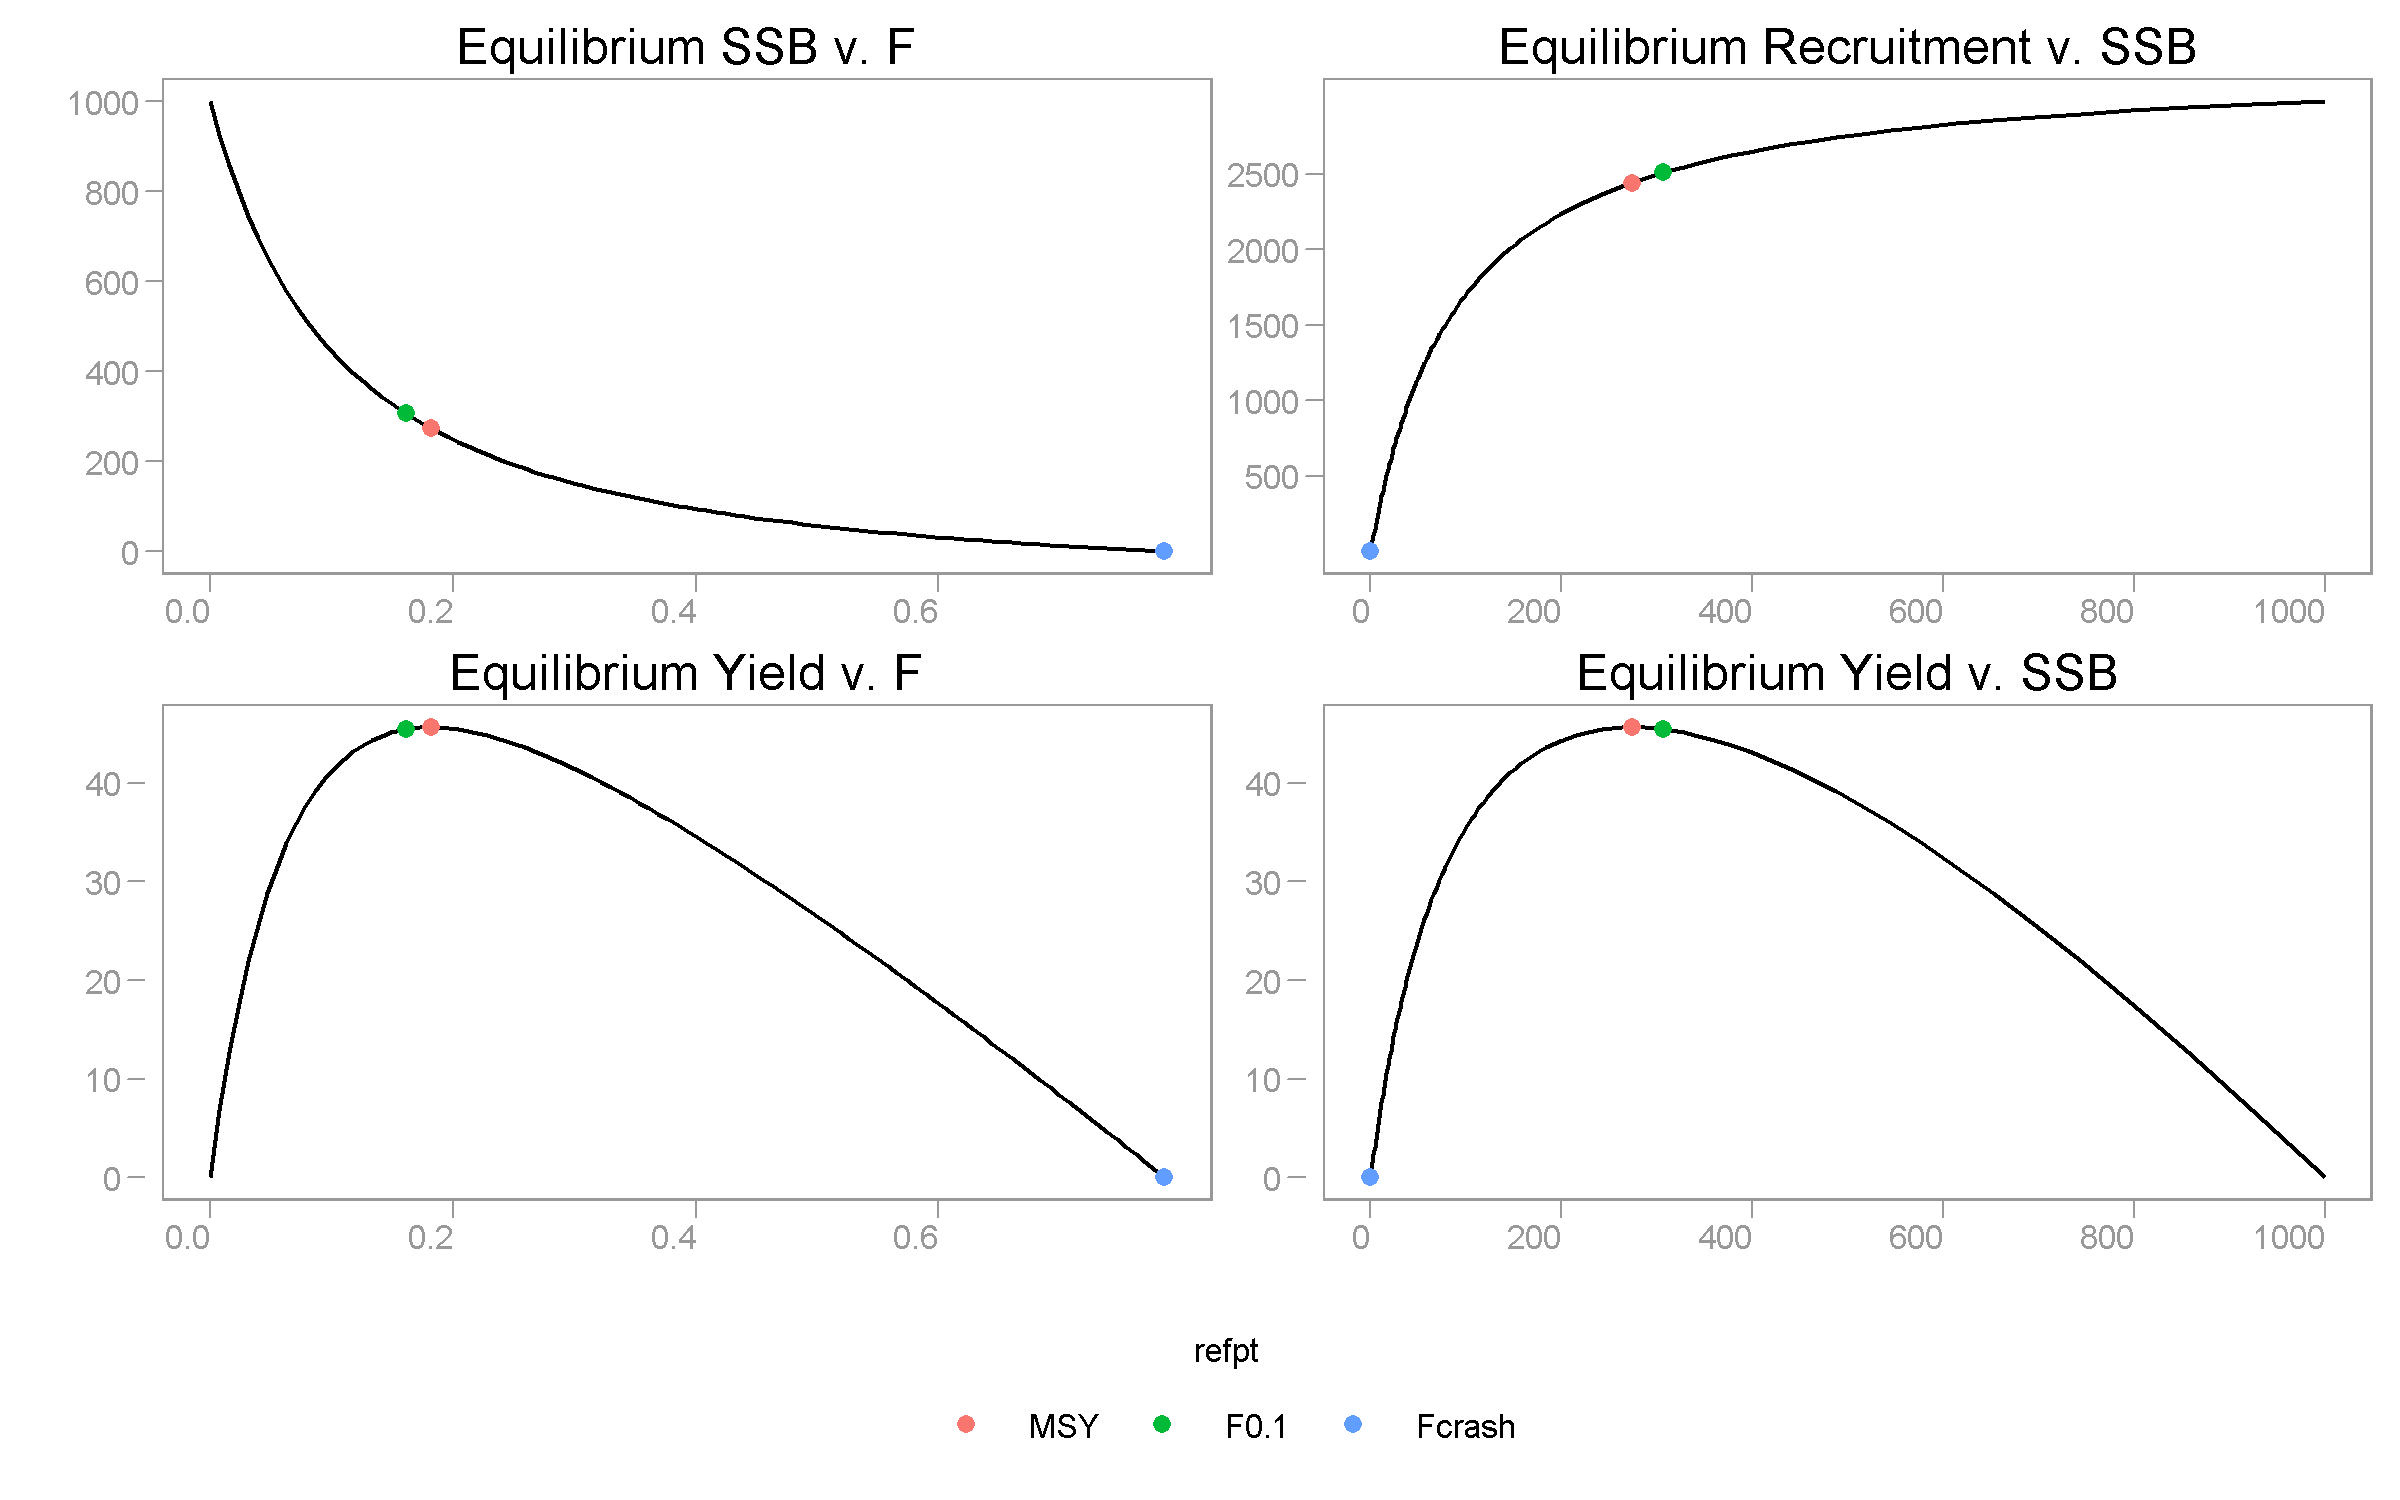
\includegraphics[width=.7\textwidth]{fig2.png}}
\end{center}
\caption{\bf{Equilibrium (i.e. expected) values of SSB and yield verses fishing mortality and recruitment and yield verses SSB; points correspond to
MSY and MSY proxies ($F_{0.1}$, $F_{Max}$, SPR30\%) and limit ($F_{crash}$) reference points.}}
\label{fig:brp}
\end{figure*}

\begin{figure*}[ht]
\begin{center}
\centerline{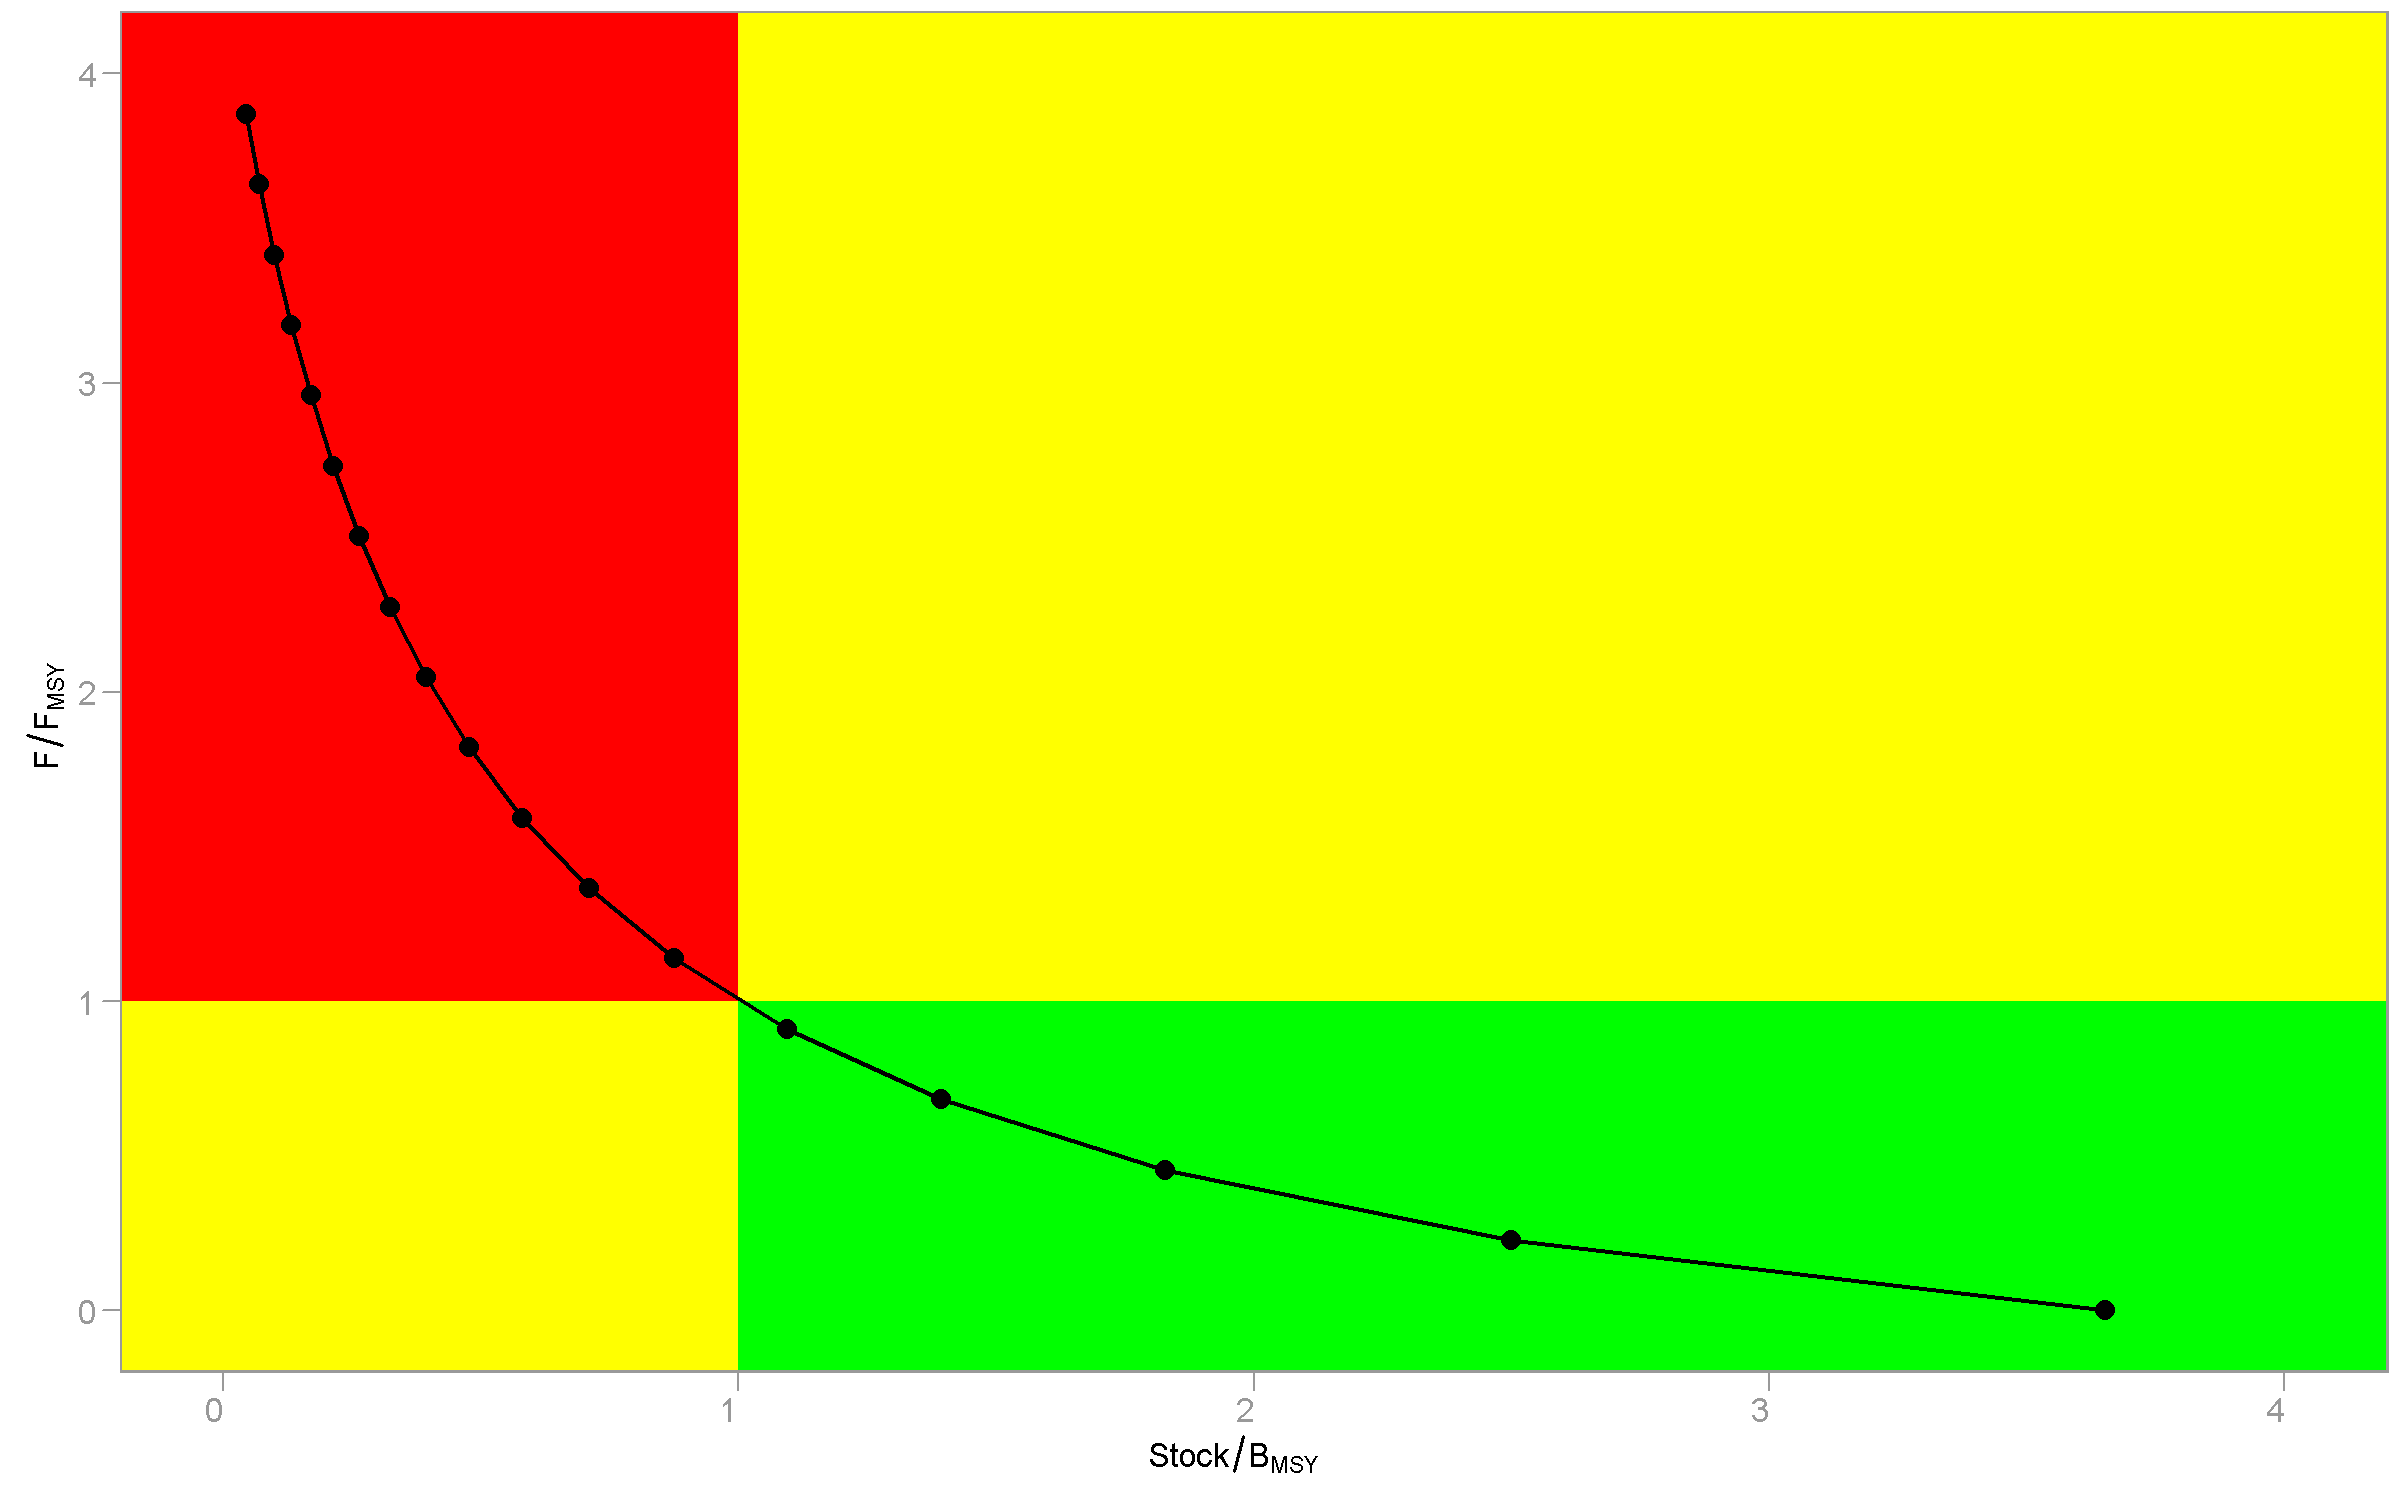
\includegraphics[width=.7\textwidth]{fig3.png}}
\end{center}
\caption{\bf{Simulated trajectories of recruitment, SSB and yield for a increasing F.}}
\label{fig:kobe}
\end{figure*}


\begin{figure*}[ht]
\begin{center}
\centerline{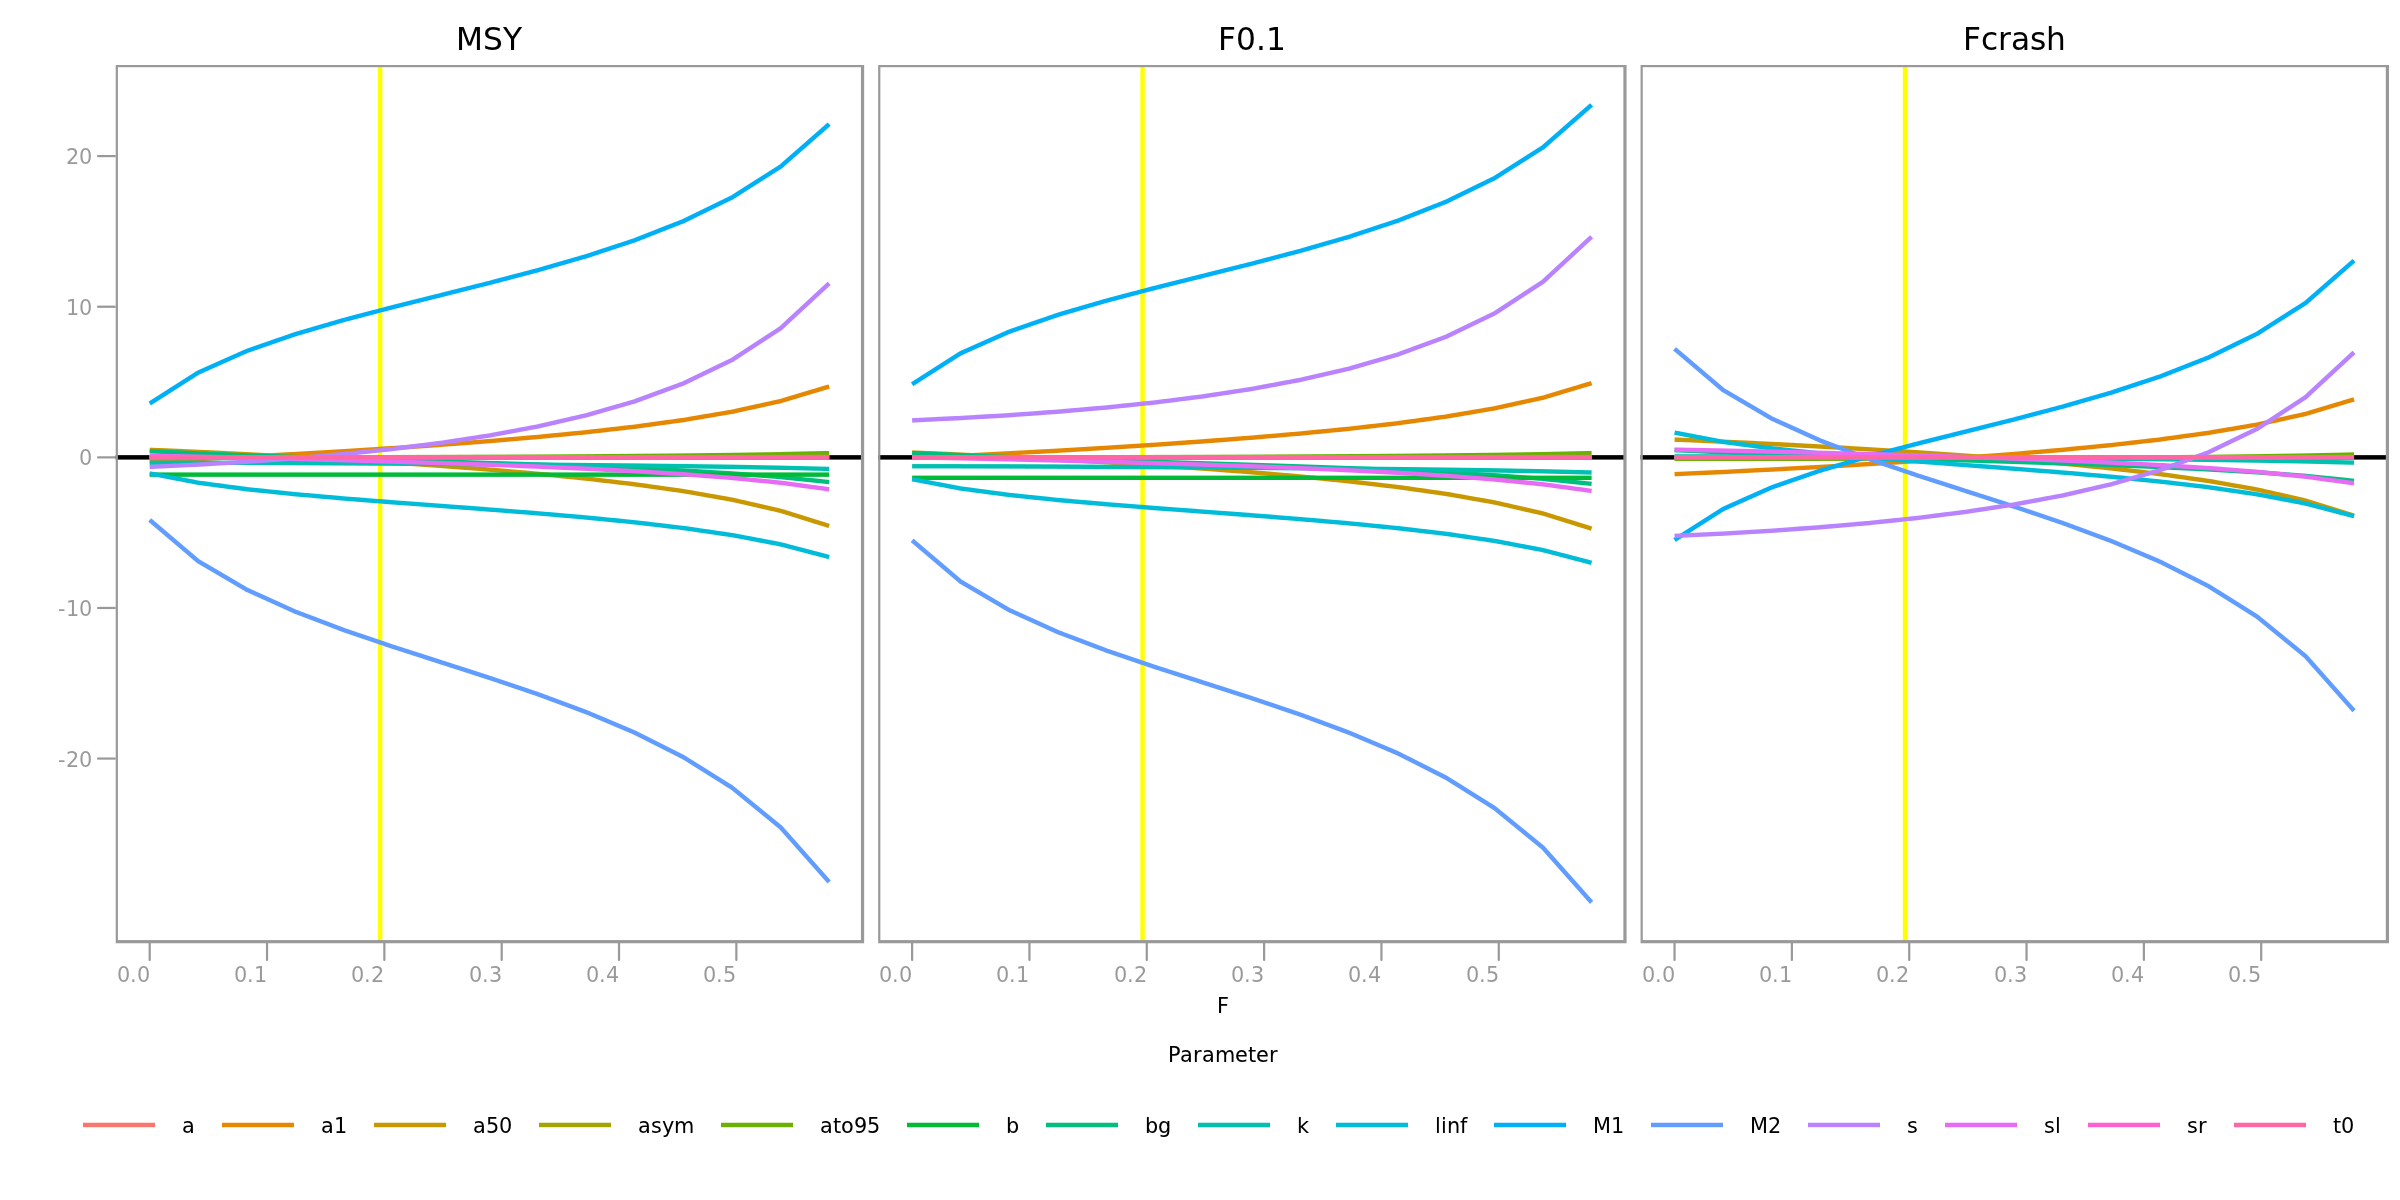
\includegraphics[width=.7\textwidth]{fig4a.png}}
\end{center}
\caption{\bf{Plots of elasticities of SSB relative to the MSY, $F_{0.1}$ and $F_{crash}$ reference points.}}
\label{fig:elasssbAll}
\end{figure*}


\begin{figure*}[ht]
\begin{center}
\centerline{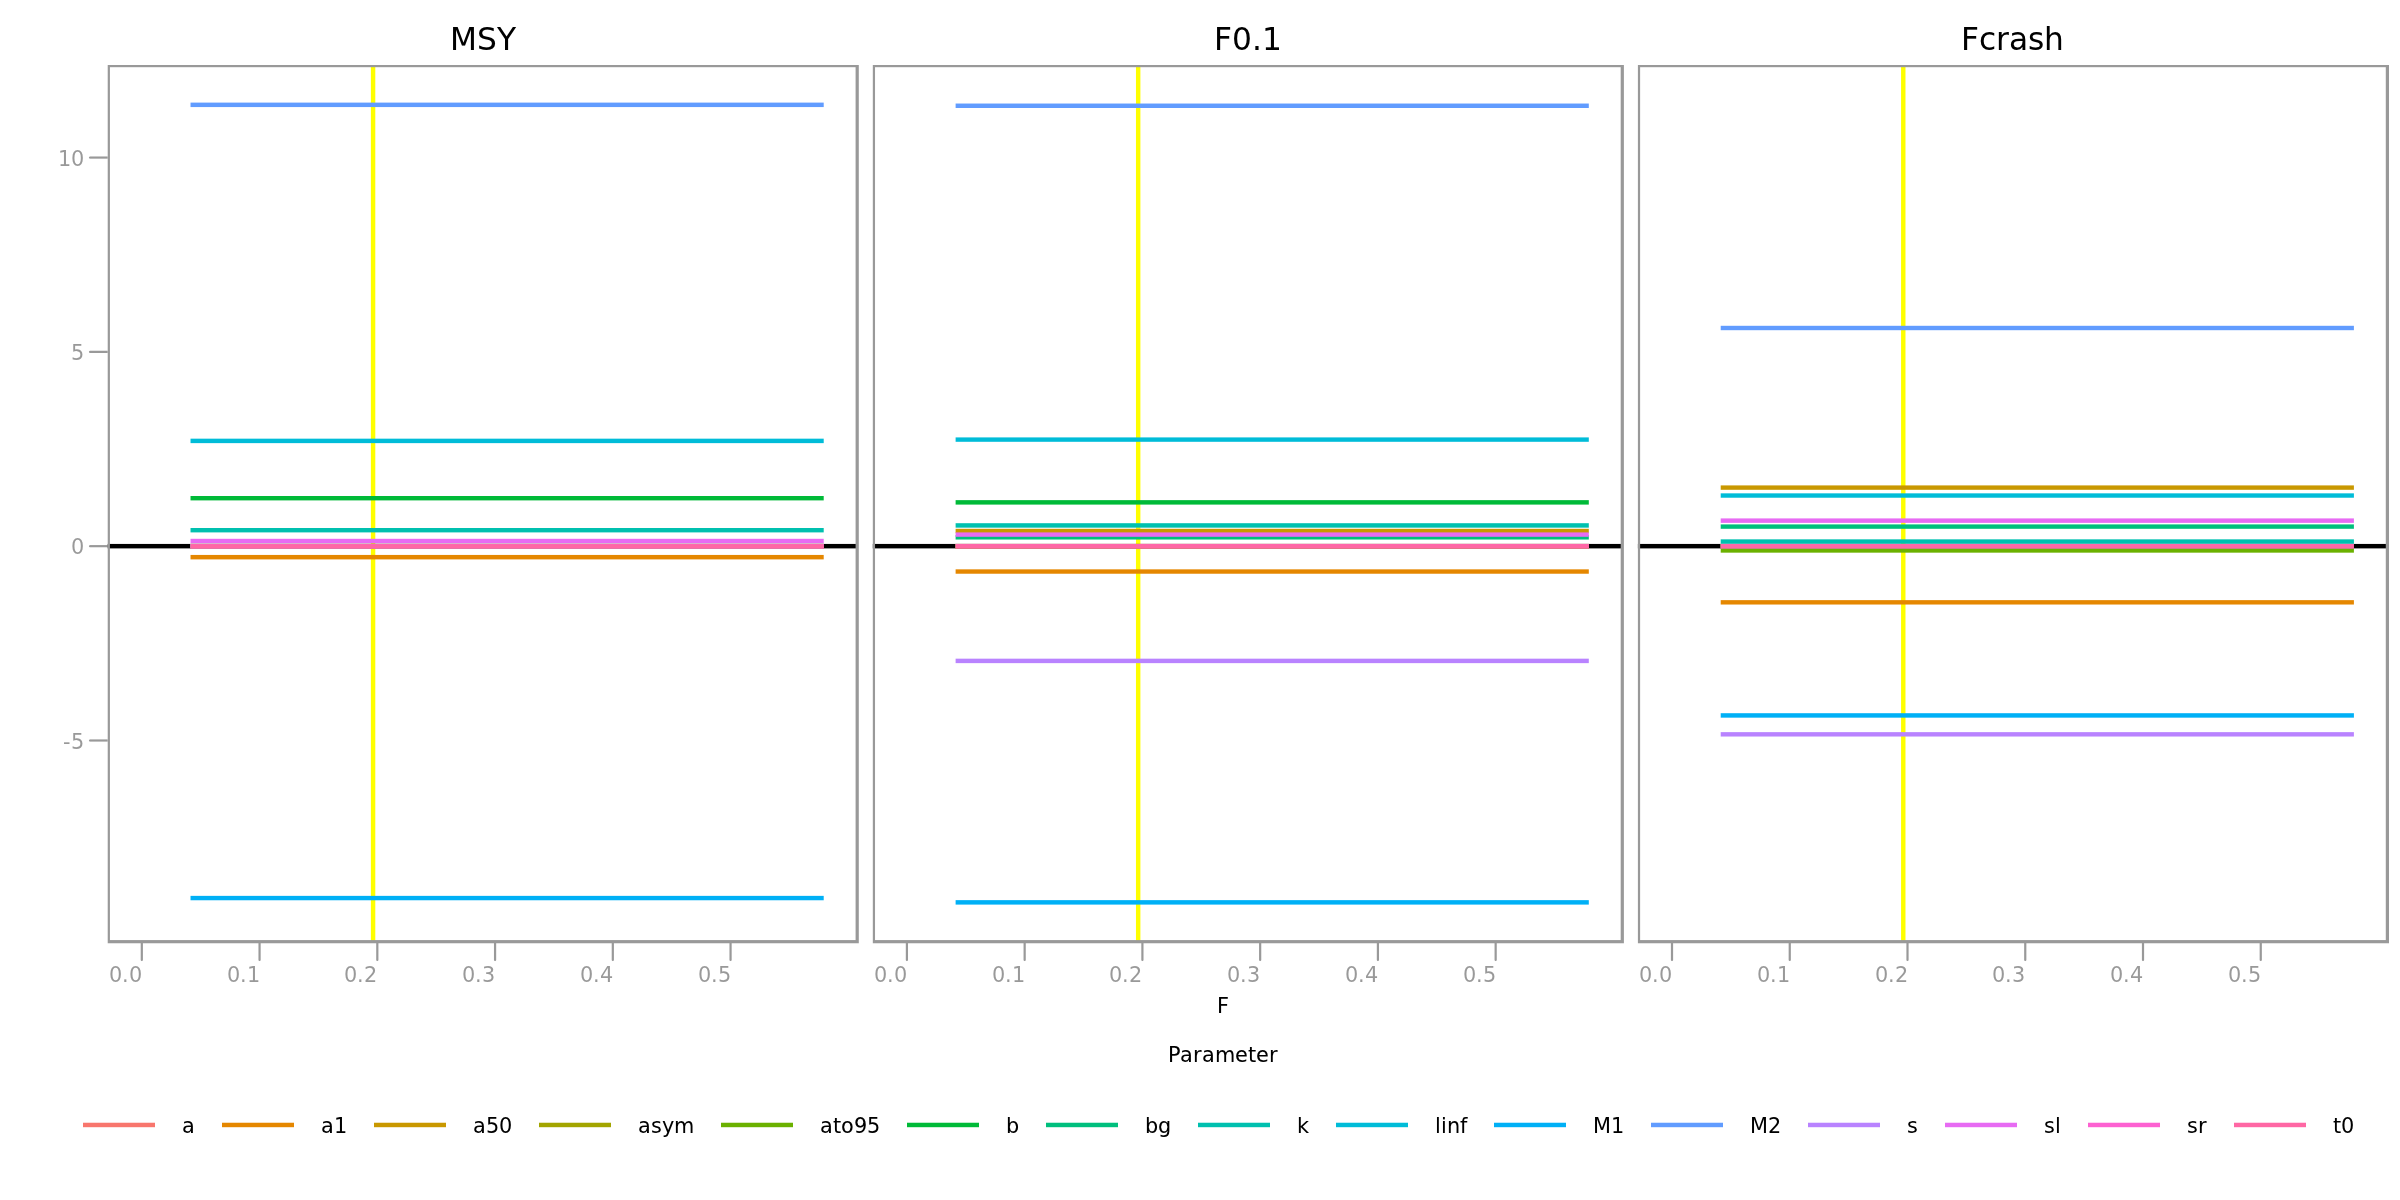
\includegraphics[width=.7\textwidth]{fig5a.png}}
\end{center}
\caption{\bf{Plots of elasticities of F relative to the MSY, $F_{0.1}$ and $F_{crash}$ reference points.}}
\label{fig:elasfAll}
\end{figure*}


\begin{figure*}[ht]
\begin{center}
\centerline{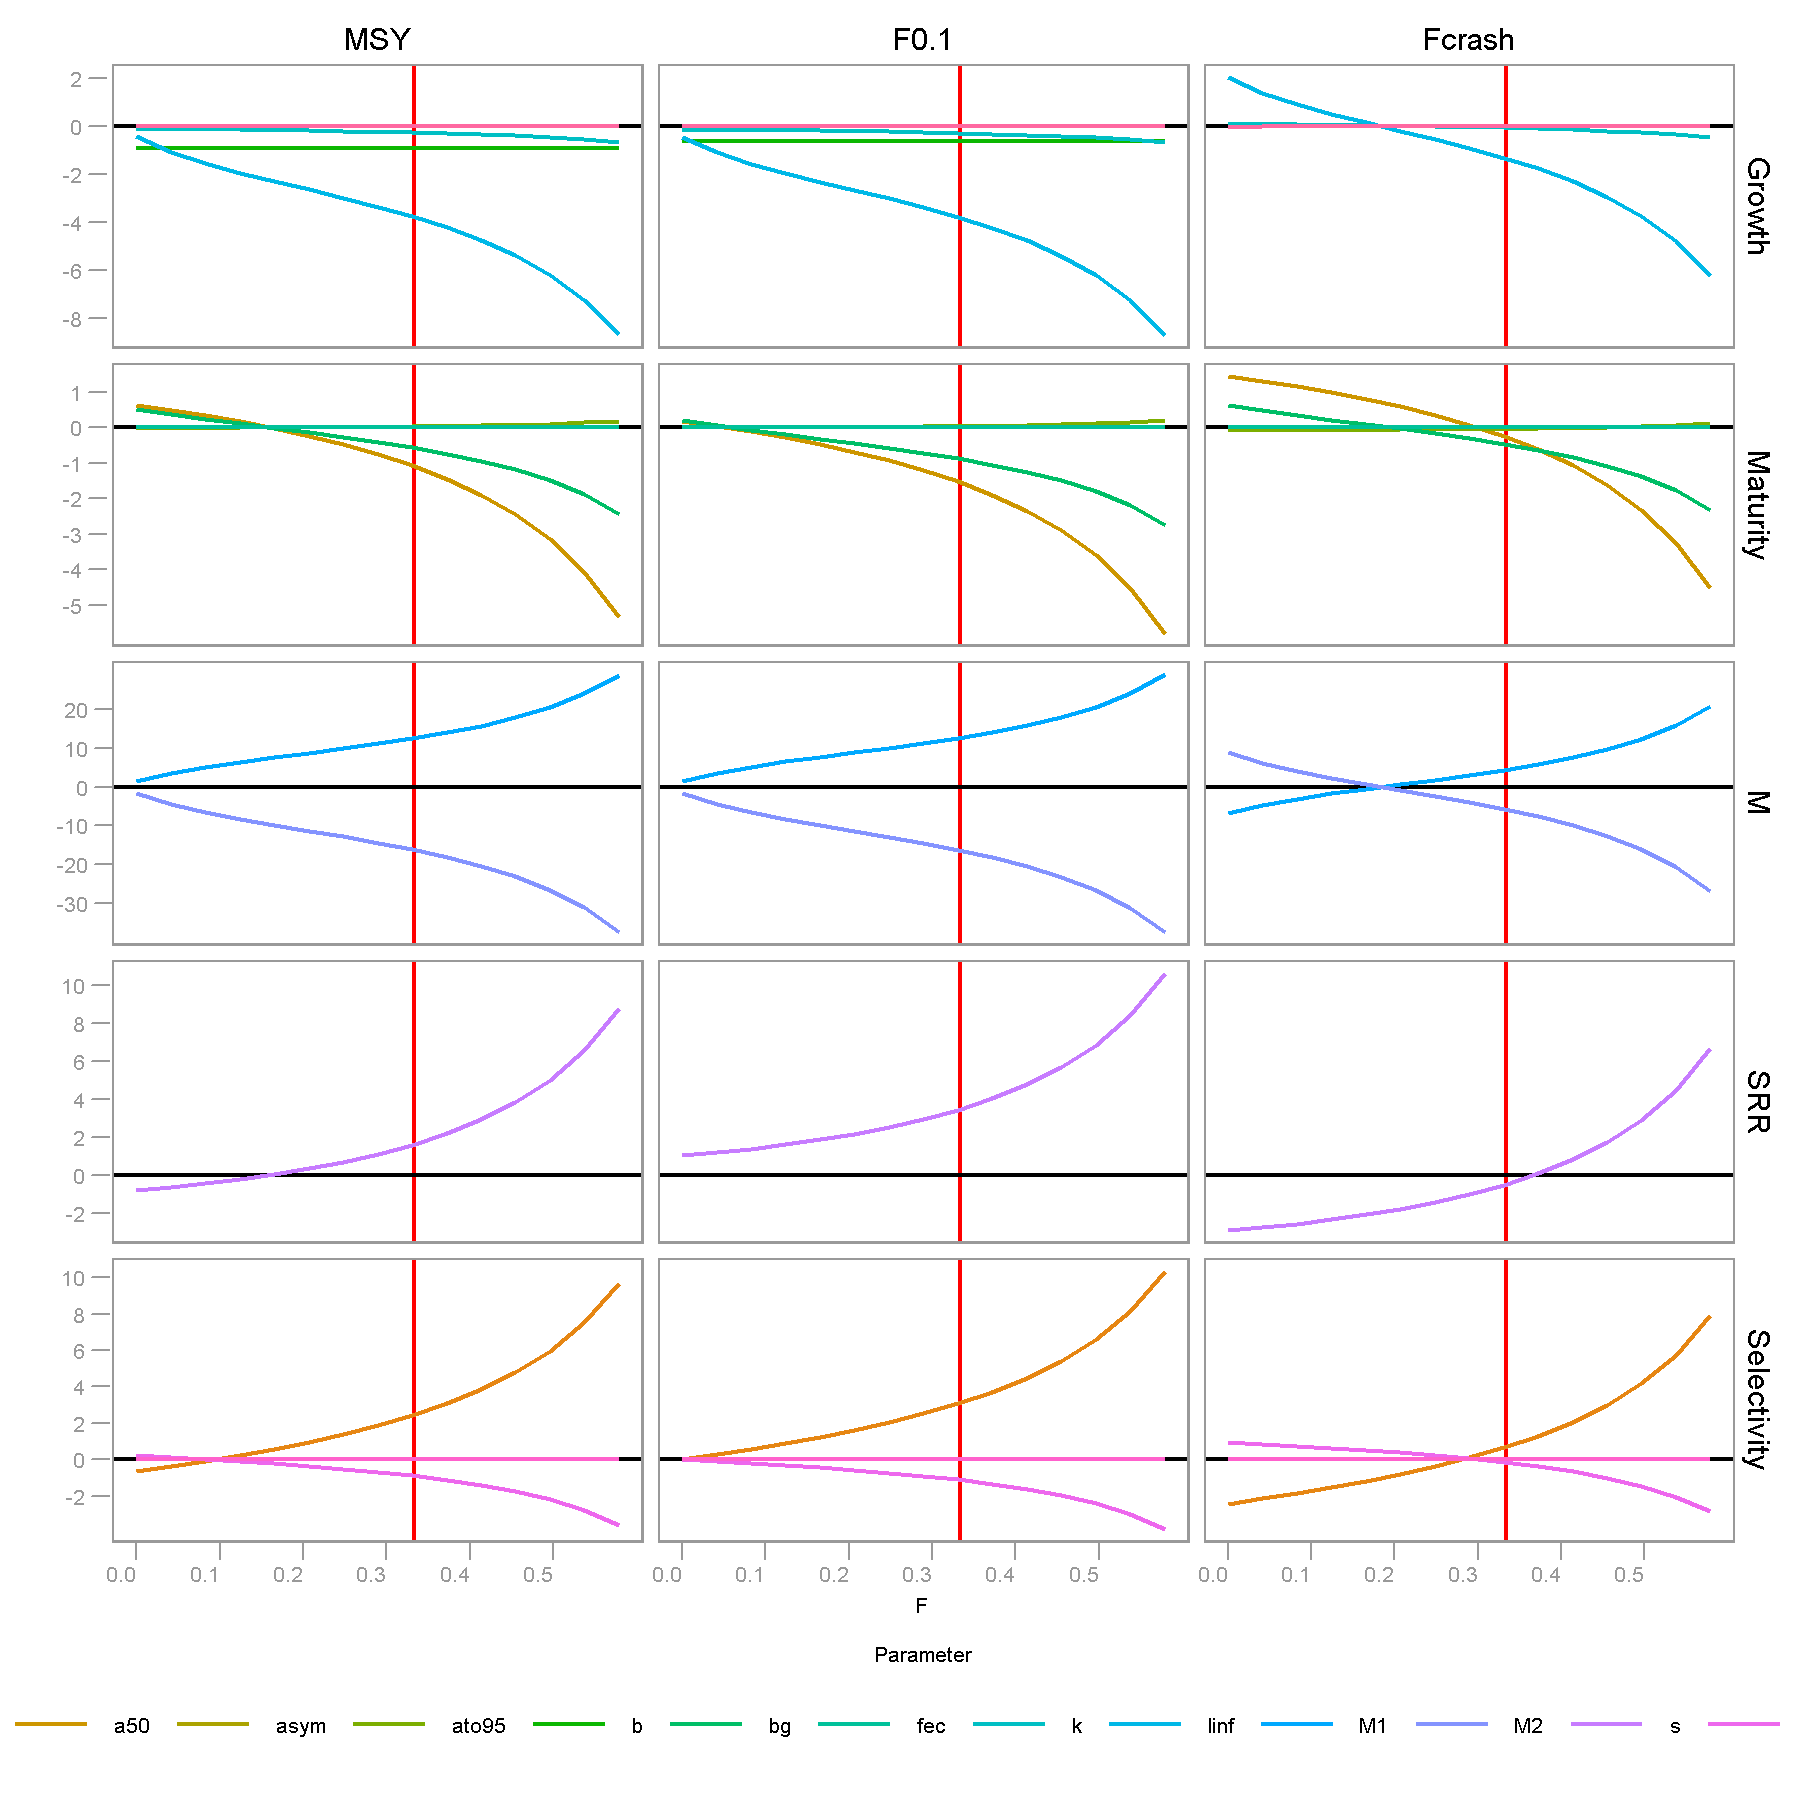
\includegraphics[width=.7\textwidth]{fig4.png}}
\end{center}
\caption{\bf{Plots of elasticities of SSB relative to the MSY, $F_{0.1}$ and $F_{crash}$ reference points.}}
\label{fig:elasssb}
\end{figure*}

\begin{figure*}[ht]
\begin{center}
\centerline{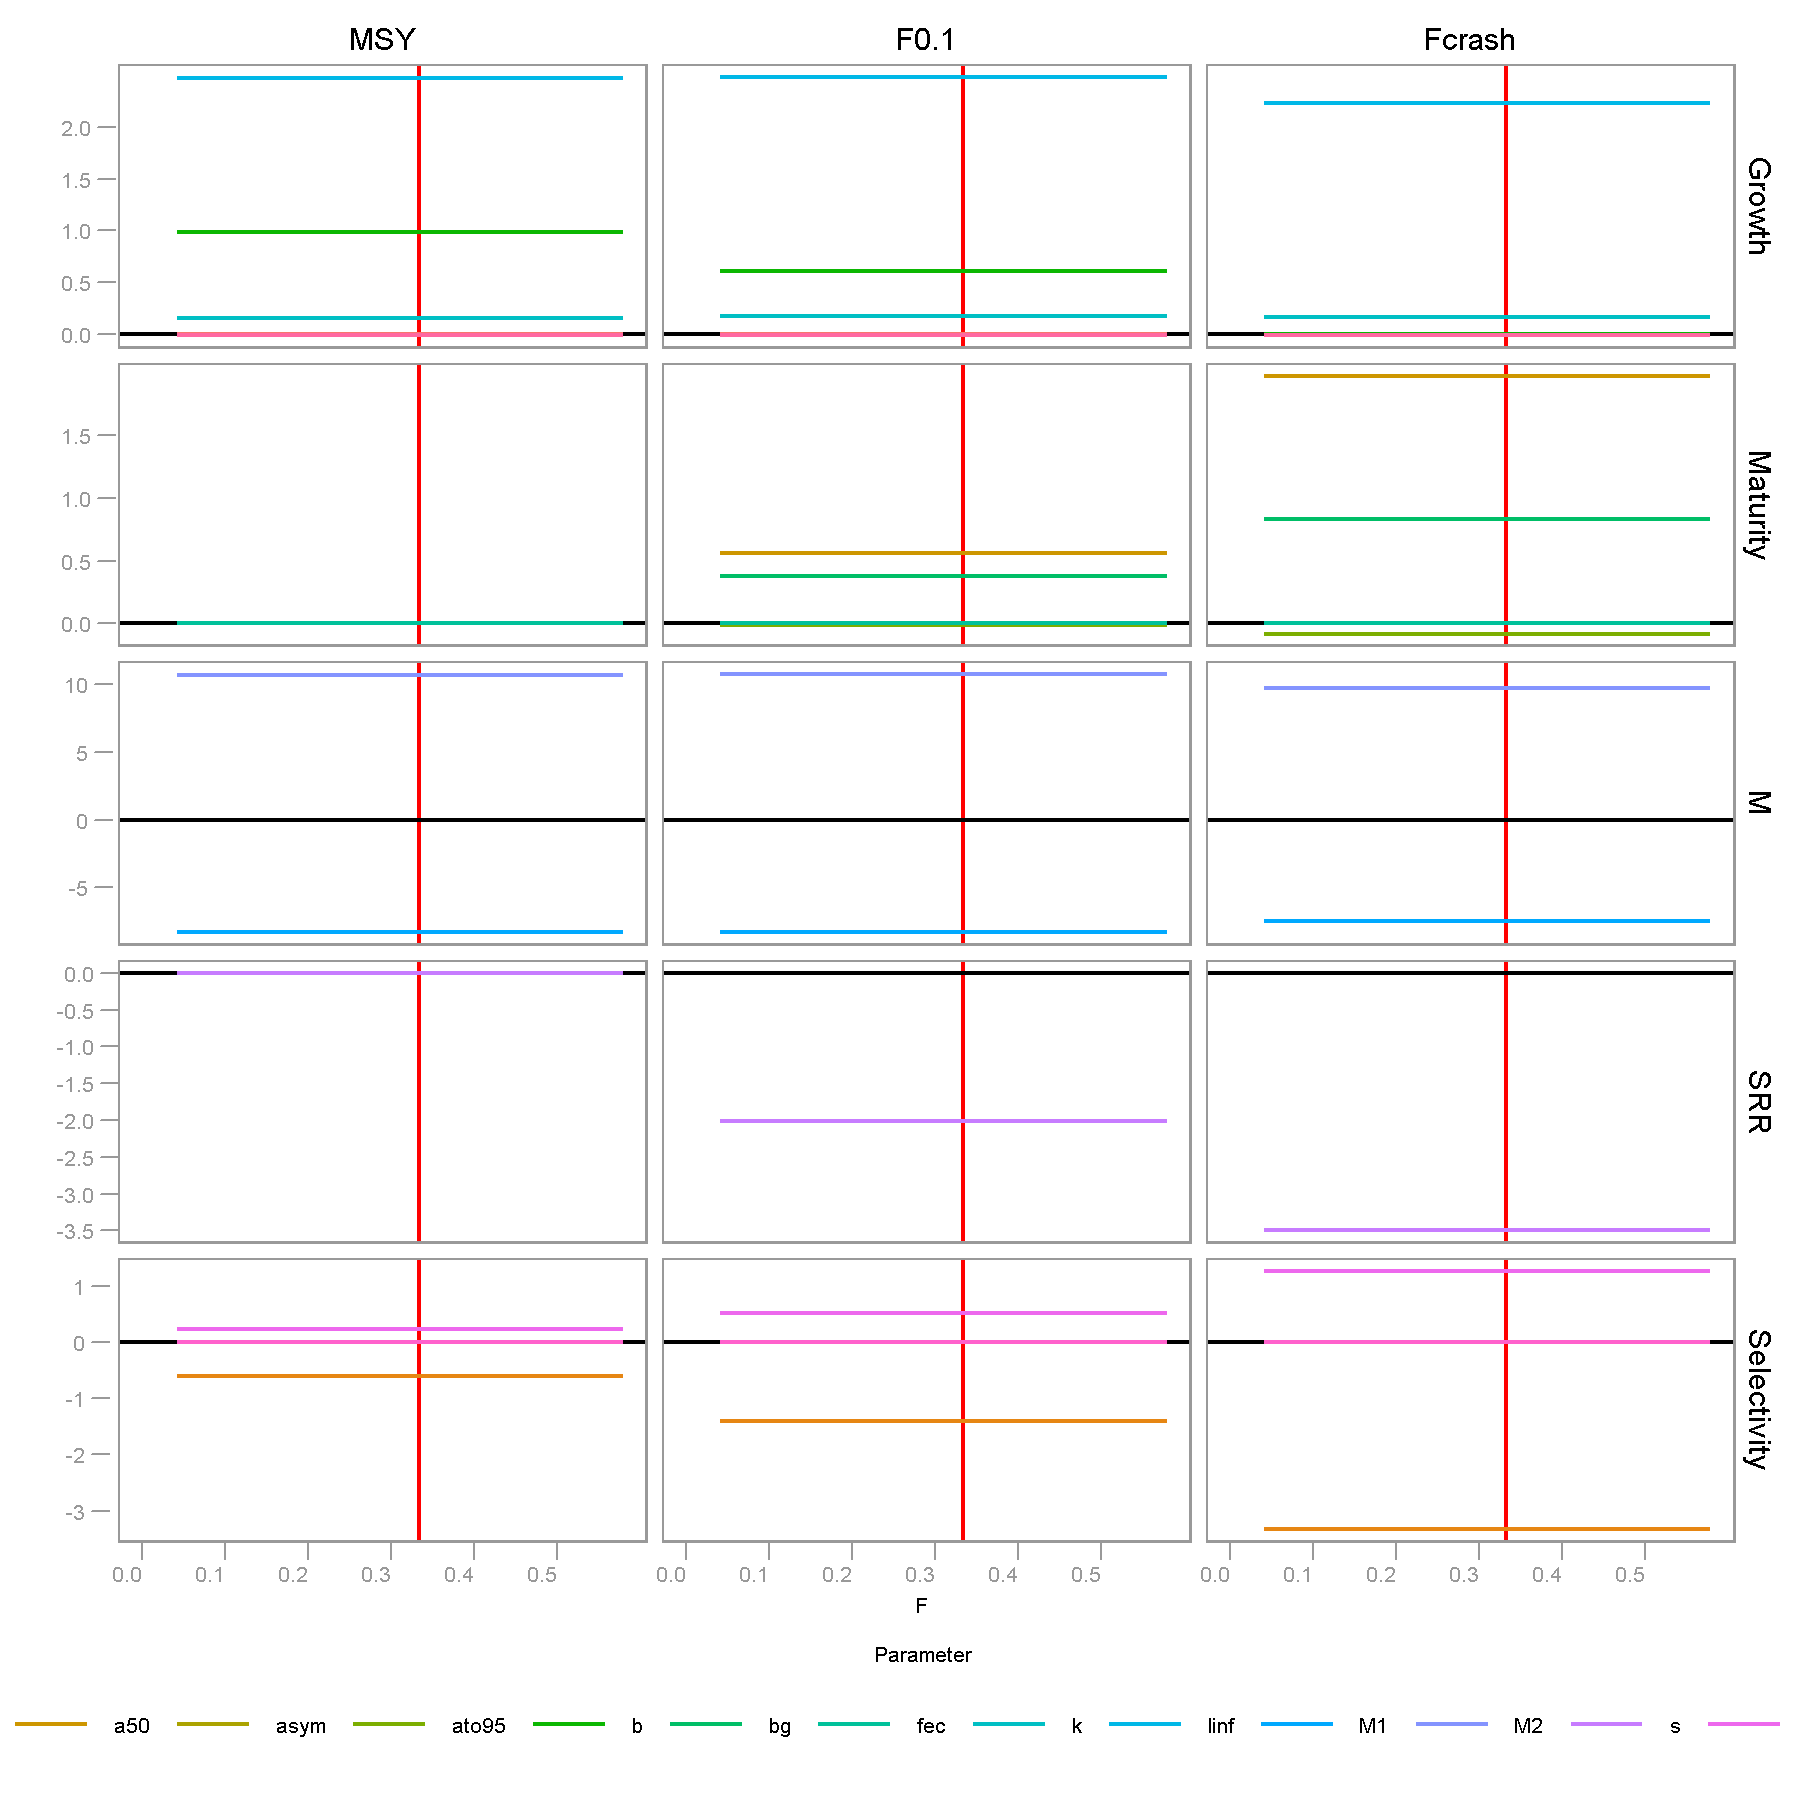
\includegraphics[width=.7\textwidth]{fig5.png}}
\end{center}
\caption{\bf{Plots of elasticities of F relative to the MSY, $F_{0.1}$ and $F_{crash}$ reference points.}}
\label{fig:elasf}
\end{figure*}


\end{document}


